% Compile with XeLaTeX or LuaLaTeX
\documentclass[10pt,a4paper]{article}
\usepackage{xcolor}
\usepackage{titlesec}
\usepackage{fontspec}
\defaultfontfeatures{Mapping=tex-text}
\usepackage{xunicode}
\usepackage{xltxtra}
\usepackage{polyglossia}
\usepackage{indentfirst}             % 段首缩进

\setdefaultlanguage{english}
% 设置字体
\setsansfont{Calibri}
\setmainfont[BoldFont=SimHei]{STKaiti}
\usepackage{amsmath}
\usepackage{amsfonts}
\usepackage{amssymb}
\usepackage{graphicx}
% 设置页边距
%\usepackage[left=2cm,right=2cm,top=2cm,bottom=2cm]{geometry}
% MATLAB代码插入包
\usepackage{listings}
\usepackage[framed,numbered,autolinebreaks,useliterate]{mcode}
% 新定义字体
\newfontfamily\song{SimSun}          % 宋体
\newfontfamily\hei{SimHei}           % 黑体
\XeTeXlinebreaklocale "zh"           % 中文断行

% Define light and dark Microsoft blue colours
\definecolor{MSBlue}{rgb}{.204,.353,.541}
\definecolor{MSLightBlue}{rgb}{.31,.506,.741}
% Define a new fontfamily for the subsubsection font
% Don't use \fontspec directly to change the font
\newfontfamily\subsubsectionfont[Color=MSLightBlue]{Times New Roman}
% Set formats for each heading level
\titleformat*{\section}{\Large\bfseries\sffamily\color{MSBlue}}
\titleformat*{\subsection}{\large\bfseries\sffamily\color{MSLightBlue}\song}
\titleformat*{\subsubsection}{\itshape\subsubsectionfont}

\author{郭大为\footnote{email: guodw3@mail2.sysu.edu.cn}\\[2ex]
    国立交通大学应数系\\[2ex]}
\title{Homework \uppercase\expandafter{\romannumeral4}}
\date{November 16, 2015}
\begin{document}

%%%% 段落首行缩进两个字 %%%%
\makeatletter
\let\@afterindentfalse\@afterindenttrue
\@afterindenttrue
\makeatother
\setlength{\parindent}{2em}  %中文缩进两个汉字位

\maketitle

\section{A section}
以下为正文部分,可以任意替换或删除

This is some text.

\subsection{A subsection 演示插入MATLAB代码}
各级标题效果演示
\subsubsection{A subsubsection}
演示代码插入效果:
\begin{lstlisting}[title=sd\_method.m, frame=shadowbox]
point = [9; 1];
H = [1, 0; 0, 9];
figure
ezcontour('x^2/2+9*y^2/2',[-9, 9, -6, 6])

% steptest decent method
sdm_points = [9; 1];
count = 0;
while(norm(point) > 1e-5)
    count = count + 1;
    g = [point(1); 9*point(2)];
    point = point - g'*g/(g'*H*g).*g;
    sdm_points = [sdm_points, point];
end
hold on
plot(sdm_points(1, :), sdm_points(2, :),'-','LineWidth',3);
count
\end{lstlisting}
图片插入效果图:
    \begin{center}
		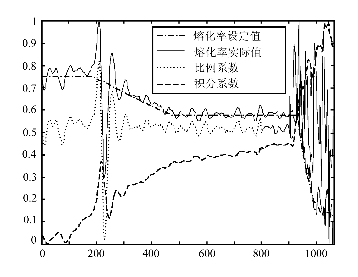
\includegraphics[width=1\textwidth]{1.eps}
	\end{center}
\end{document}
